\documentclass[../main/thesis.tex]{subfiles}

% Overleaf graphics path
\graphicspath{{thesis/methodology/figures/}}

% Local graphics path
% \graphicspath{{/home/arefk/uio/MScThesis_AreKvanum2022_SeaIceML/thesis/methodology/figures/}}


\begin{document}
\section{Methodological framework}
This Section will outline the theoretical background of convolutions from a deep learning point of view, as well as provide a brief overview of image segmentation as a computer vision task. Furthermore, the Methodological framework required to develop the U-Net architecture will be highlighted, followed by the description of a training loop and the central algorithms utilized. Finally, validation metrics used to asses the performance of the developed deep learning system will be derived.

\subsection{Convolutional layers}
\label{sec:convolutional-layer}
Convolutional layers incorporated into a deep neural network which utilized the backpropagation algorithm \citep{Rumelhart1986} was initially proposed by \citep{LeCun1989} to classify handwritten numbers. The layer \citet{LeCun1989} presented consists of an arbitrary amount of filters, which are small two dimensional matrices (e.g. $(3 \times 3)$ pixels) designed to capture a certain structure in the image such as lines or edges \todo{Sitere boka til Goodfellow2016?}. Each filter contains trainable weights, which are learned from the data during backpropagation \citep{LeCun1989} and gradient descent. When a filter is convolved with all possible local neighborhoods from the input, it outputs a feature map which represent where the input image triggered a response from the filter \citep{Zeiler2010}. Moreover, inputting feature maps to a convolutional layer allows for the filters to respond to combinations of lower level structures, which trains the layer to detect more complicated patterns \citep{Fukushima1980}. Additionally, stacking convolutional layers in a network-architecture structure increases the field of view for each subsequent layer, which makes each layer observe an increasingly complex pattern of higher order feature maps at increasingly larger spatial scales \citep{Fukushima1980}. As a result, convolutional layers are able to discern between object and background as they percieve only a limited view of the scene. The convolutional layer is also invariant to translation of the object, since the filter is constant when creating the feature map \citep{LeCun1989}. I.e. the filter is detecting the same feature at all locations in the image, known as weight sharing \citep{LeCun1989}.

The number of trainable parameters for a convolutional layer is equal to the size of a filter times the number of filters. As a result, the number of trainable parameters is invariant to the spatial extent of the input images. On the other hand, fitting a fully connected layer to spatial gridded data consists of associating a separate trainable parameter to each pixel. As such, the size of a fully connected layer scales with the size of the image, which increases the risk of overfitting the network. In the case of the convolutional layer, \citet{LeCun1989} notes that reducing the number of trainable parameters through weight sharing constrains the solution space such that overfitting is avoided while still having enough trainable parameters to fit the layer to the data. Furthermore, the fully connected layer is not invariant to translation as each trainable parameter is exclusive to their respective pixel, hence no weight sharing. As such, the layer is unable to detect a similar object at a different position, reducing their usefulness for image-based prediction tasks.

Finally, \citet{Ciresan2012} showed that the processing time of a convolutional layer is significantly shortened by utilizing a graphics processing unit (GPU), due to their large amount of compute cores compared to traditional Central Processing Units (CPUs). Furthermore, the authors of \citet{Krizhevsky2012} provided the first publicly available implementation of a CNN running on a GPU by utilizing the Nvidia Compute Unified Device Architecture api. \citet{Krizhevsky2012} also demonstrated that their results are tied to the performance of the GPU in terms of available memory as well as floating point operations, with the implications that a better GPU as well as larger datasets would improve their results. As such, the modern implementation of convolutional layers, and by extension deep learning architectures which stacks many convolutional layers, can be initiated with more trainable parameters since they can process greater datasets consisting of larger samples due to their GPU implementation.

The convolutional layer can be described mathematically by utilizing the previously described principle of allowing the filter to only perceive a local neighborhood of the input. Consider the value of a single point $y_{i,j} \subset Y \in{\mathbb{R}^2}$ where $i,j$ denote the position in the x and y direction as a single output from a convolution. Let $X \in{\mathbb{R}^3}$ be an input image of size $(A \times B \times D)$ consisting of a single channel, and $W \in{\mathbb{R}^3}$ be a symmetric filter of size $(r \times r \times D)$. Then, the value at a single point $y_{i,j}$ is given as follows,

\begin{equation}
    \label{eq:singlepointconv}
    y_{i,j} = \sum_{a=1-\frac{r}{2}}^\frac{r}{2} \sum_{b=1-\frac{r}{2}}^\frac{r}{2} \sum_{d=1}^D W_{a + \frac{r}{2},b + \frac{r}{2}, d} X_{i+a,j+b,d}
\end{equation}

Where the subscript notation is used in $W$ and $X$ to denote indexes similarly to $Y$. Repeating Equation (\ref{eq:singlepointconv}) across all points $x \subset X$ by applying a sliding window technique returns the convolution of X with filter W, which results in an output $Y$ with size $(A-r+1) \times (B-r+1)$. Note that the above definition only applies for $X_{1 \leq i+a \leq A, 1 \leq j+b \leq B}$. The size of the output can be adjusted by padding the input $X$ by a size $P$ in each direction or increasing the stride $S$ of the sliding window, which reformulates the output size of $Y$ in a single dimension as a function

\begin{equation}
    \label{eq:outputdim}
    Y_\text{dim} = \lfloor\frac{A - r + 2P}{S} + 1\rfloor    
\end{equation}

The convolutional layer adds the convolution described in Equation (\ref{eq:singlepointconv}) with a bias term $B \in{\mathbb{R}^2}$ of same spatial shape as $Y$, as well as applying an activation function $g$ to each $y_{i,j}$ which introduces nonlinearity. In summary, the output of a convolutional layer can be described as 

\begin{equation}
    \label{eq:outputconv}
    Y^\prime = g(Y + B) = g(W^TX + B)
\end{equation}

If the number of filters increases from $1$ to $N$, Equation (\ref{eq:outputconv}) is repeated for all filters, resulting in an output $Y \in{\mathbb{R}^3}$ of size $(Y_\text{dim1}, Y_\text{dim2}, N)$.

\subsection{Image segmentation}
\label{sec:image-segmentation}
Image segmentation is a computer vision task where pixels are assigned labels according to some predetermined rules. It is common to define an image segmentation task either as a study of countable \textit{things} (Instance segmentation), or recognizing similarly textured \textit{stuff} (Semantic segmentation) \citep{Kirillov2018}. The task for this thesis, which is labelling sea ice concentration according to its predicted concentration class, falls into the latter category following the definition of \textit{stuff} in \citet{Adelson2001}. I.e. the current task is to assign each pixel in a predicted scene a single class label.

Network architectures based on the Convolutional Neural Network (CNN) \citep{LeCun1989,Ciresan2012,Krizhevsky2012,Simonyan2014,Szegedy2014,He2015a,Huang2016} can be used to perform pixelwise semantic segmentation, however the CNN architectures listed have been developed for image classification i.e. predicting a single label for the entire image. \citet{Ciresan2012a} presented an approach where a CNN (see the architecture of \citet{Ciresan2012}) was used to predict a label for all pixels in an image. Instead of processing the entire image at once, \citet{Ciresan2012a} applied a sliding window technique which predicted each pixel by using their surrounding neighborhood as input. However, due to only processing parts of the image at once, the segmentation algorithm in \citet{Ciresan2012a} is computationally expensive as the CNN must be run for all neighborhoods as well as limiting the context in which each pixel is classified in to a surrounding local context \citep{Ronneberger2015}.

To capture the global context of a scene, network architectures such as \citet{Long2015,Noh2015,Ronneberger2015,Badrinarayanan2017,Chen2018} implement the Encoder-Decoder architecture, where the entire input scene is first processed by a CNN-like architecture referred to as the Encoder to produce a signal. The signal is then used as input to a subsequent network which reconstructs the encoded signal to match the resolution of the original image through upsampling. \citet{Long2015,Ronneberger2015,Badrinarayanan2017} all apply the Deconvolution architecture proposed by \citet{Zeiler2010} to upsample the encoded signal through the use of a trainable deconvolutional layer, which will be described in greater detail in Subsection (\ref{sec:tconv}). However, other upsampling techniques exists, such as unpooling used in \citet{Noh2015} which undoes a maxpool (downsampling) layer (maxpooling is described in Subsection (\ref{sec:maxpool})).

This thesis will utilize the U-Net architecture proposed by \citet{Ronneberger2015}. The U-Net was originally developed for medical image segmentation, however the architecture has shown promising results for both pan-arctic seasonal \citep{Andersson2021} and regional short term \citep{Grigoryev2022} sea ice concentration forecasting amongst other applications. Another aspect which makes the U-Net more suitable to the current task, compared to other previously mentioned image-to-image architectures is that the network converges quickly, which is ideal when working with a dataset consisting of few samples \citep{Ronneberger2015}.

\subsection{Describing the U-Net architecture}
Figure (\ref{fig:unet-overview}) shows the U-Net architecture. This section intends to describe the different components constituting the architecture from a technical point of view. 

\begin{figure}
    \centering
    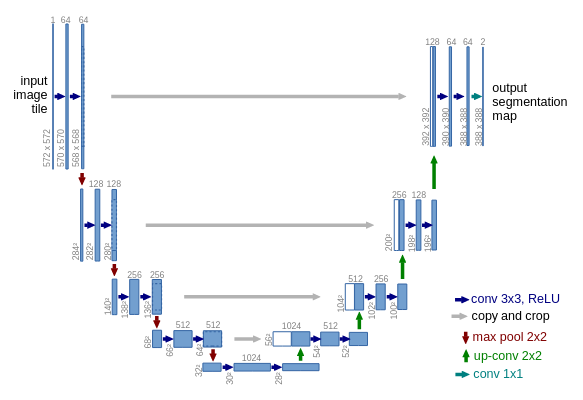
\includegraphics[width=0.9\textwidth]{unet_screenshot}
    \caption{\label{fig:unet-overview}The U-Net architecture. The blue boxes represent feature maps, with the lower left numbers determining the spatial resolution and the top number the amount of feature maps. White boxes in the expansive path (right side / decoder) are the copied feature maps from the contractive path (left side / encoder). Arrows denote the different operations. Note that the original U-Net only performs \textit{valid} convolutions, i.e. convolution without padding to match the input. This causes a convolutional layer to slightly decrease the spatial extent. As a result, the copied features from the contracting path are also cropped to match the dimensionality in the expansive path. Figure extracted from \protect\citet{Ronneberger2015}.}
\end{figure}

\subsubsection{The convolutional block}
A single convolutional block consists of two repeat convolutional layers, each followed by the Rectified Linear Unit (ReLU) nonlinear activation function, which is defined as $f(x) = \max{(0,x)}$ \citep{Nair2010}. Each convolution is performed using a $3 \times 3$ window. The original formulation of the U-Net also does not apply padding to the input, resulting the convolutional filter only being applied to the entries of the input where the filter is never out of bounds. With a stride of $S=1$, this results in each convolutional layer reducing the spatial extent by two pixels in each direction following Equation (\ref{eq:outputdim}). It is also noted that the number of feature maps is doubled after each downsampling step, which is performed by the pooling layers.

\subsubsection{Maxpooling}
\label{sec:maxpool}
Pooling operations are used to reduce the spatial extent of the current feature maps, by downsampling the data in the spatial dimensions. As seen in Figure (\ref{fig:unet-overview}), the U-Net downsamples the data in the contracting path through $2 \times 2$ maximum pool layers with a stride of 2. This specific configuration causes the spatial resolution to be halved. In the max-pool layer, a filter runs through each input channel and and chooses the maximum value inside the neighborhood of the filter. As such, the extreme values in each feature map is retained at the expense of rejecting the rest of the data. Since the maxpooling operation is rejecting some parts of the data, it may be regarded as a regularizer for the network which aid in avoiding overfitting.  See Figure (\ref{fig:maxpool}) for a graphical description.

\begin{figure}
    \centering
    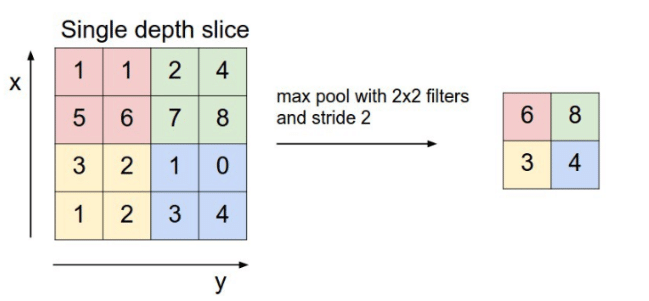
\includegraphics[width=0.9\textwidth]{The-MaxPool-operation}
    \caption{\label{fig:maxpool}The max-pool operation for a $2 \times 2$ filter with a stride of 2. Figure taken from \protect\citep{MihaiDaniel2020}}
\end{figure}

\subsubsection{Transposed convolutions}
\label{sec:tconv}
Transposed convolution was proposed by \citet{Zeiler2010} (note the incorrect use of deconvolution, this is not the mathematical inverse of a convolution) to increase the resolution of a feature map. The method was first utilized by \citet{Long2015} to connect the coarse output of an encoder with the image resolution of the target (it is referred to as both \textit{backwards convolution} and \textit{deconvolution} in the proceedings paper). Similar to the convolutional layer, the transposed convolutional layer involves striding a convolutional filter with trainable parameters across a feature map. However, the transposed convolutional layer projects a singular entry from the input through the convolutional kernel to produce an output that is larger than the input.

In the Encoder architecture, lower level feature maps provide spatial information regarding where stuff is located in a scene, whereas higher level feature maps contain information regarding what is in the scene at the expense of losing spatial information \citep{Long2015}. To circumvent this, \citet{Ronneberger2015} concatenate the features from the contracting path with the output from the transposed convolution at the same level of depth, i.e. where the number of feature maps are equal at the end of the convolutional block. The concatenation operation is possible in \citet{Ronneberger2015} since they crop the feature maps in the encoder in their spatial dimensions to match the spatial dimensionality of the feature maps in the decode. The operation can be seen in Figure(\ref{fig:unet-overview}) denoted by the gray arrow. The resulting convolutional layer is then trained to make a more precise prediction due to the concatenated input \citep{Ronneberger2015}.

\subsubsection{Outputs}
The output layer of the U-Net is denoted by the turquoise arrow at the right side of Figure (\ref{fig:unet-overview}). The arrow denote that the input processed by a convolutional layer with a number of filters equal to the number of output classes. Each filter is of size $(1 \times 1)$ and maps each layer in the input feature map to their respective class probability map of equal spatial shape \citep{Ronneberger2015}. By inspecting Figure (\ref{fig:unet-overview}), the U-Net outputs two feature maps, and from each feature map the pixelwise probability of belonging to the associated class can be computed.

\subsection{Training procedure for the U-Net}
This subsection aims to demonstrate how \citet{Ronneberger2015} trained the U-Net, and will consequently highlight some different hyperparameters and exemplify some functions and operations which are used performed training. Hyperparameters refer to model parameters which are not updated during training \citep{Yu2020a}, and may directly influence the model architecture or the training procedure. This section will not describe how samples were preprocessed and loaded, and modifications made which reflects concerns regarding medical images may be noted but not explained.

Training the U-Net start by assigning random values to the weights of the network. Since the U-Net utilizes the ReLU activation function after each convolutional layer in the convolutional blocks \citep{Ronneberger2015}, it is standard for each layer to draw the weights from a normal distribution with $\mu = 0$ and standard deviation $\sigma = \sqrt{\frac{2}{n_l}}$, where $n_l$ is the number of inputs to the layer \citet{He2015}. This weight initialization scheme ensures that variance of the feature maps are approximately equal, i.e. avoids varying the activation of input signals between layers \citet{He2015,Ronneberger2015}.

The process of training the U-Net involves making predictions on all training data. For each sample, what is predicted is compared against a ground truth label associated with the sample. For the U-Net, a pixelwise prediction map is created by computing the pixelwise softmax which is an extension of the softmax function \citep{Bridle1990} defined as 

\begin{equation}
    \label{eq:psoftmax}
    p_{k,i,j} = \frac{e^{a_{k,i,j}}}{\sum_{k^{\prime} = 1}^Ke^{a_{k^\prime,i,j}}}
\end{equation}

where $a_k$ is the feature map for feature channel $k$ of input $x$ and $K$ is the number of output classes. $i,j$ is the spatial coordinates. Similarly to the standard softmax function \citep{Bridle1990}, Equation (\ref{eq:psoftmax}) is $\approx 1$ for the class that has maximum $a_{k,i,j}$ and $\approx 0$ for all other classes, albeit depthwise in the channel dimension for all pixels \citep{Ronneberger2015}.

To quantify the prediction error, a loss function is defined. The overall goal of training a neural network is to minimize the loss function with respect to the trainable weights. For the U-Net, a weighted variation of the cross entropy loss function is proposed \citep{Ronneberger2015}. 

\begin{equation}
    L(p) = \sum_{i,j \subset \mathbb{Z}^2}w_{i,j}log(p_{l,i,j})
\end{equation}

where $w$ is a predefined weight map and $p_{l,i,j}$ is the prediction made at pixel $i,j$ at the true label $l$.

The error computed by the loss function is then sent backwards throughout the network according to the backpropagation algorithm \citep{Rumelhart1986}, which effectively computes the gradient of the loss function with regards to the trainable parameters 
\begin{equation}
    \label{eq:weight_adjust}
    \frac{\partial L}{\partial w_l} = \frac{\partial L}{\partial p}\frac{\partial p}{\partial w_l}
\end{equation}
where $w_l$ is the trainable parameters associated with the $l$-th layer. The gradient of the loss for a weight at a given layer shown in Equation (\ref{eq:weight_adjust}) is used by an optimizer to adjust the weights such that the loss is minimized with respect to the weights (gradient descent).

\citet{Ronneberger2015} uses the stochastic gradient descent with momentum optimizer implemented in the Machine Learning library Caffe \citep{Jia2014}, where the optimizer is defined as follows,

\begin{equation}
    \label{eq:msgd}
    w_l^{t+1} = \gamma(w_l^t - w_l^{t-1}) - \mu\frac{\partial L}{\partial w_l^t}
\end{equation}

In Equation (\ref{eq:msgd}), the superscript $t$ was added to $w$ and refers to training step, which is defined as a prediction and subsequent backpropagation of a batch of samples, where the size of a batch is a pre-determined hyperparameter. $\gamma$ and $\mu$ are the momentum and learning rate hyperparameters respectively. Note that $\gamma$ is introduced by momentum stochastic gradient descent, whereas the learning rate $\mu$ is a hyperparameter common for all deep learning models and determines the rate of weight adjustment as seen in Equation (\ref{eq:msgd}).

When all training samples have been inspected once by the U-Net, the training data is shuffled and the above outlined training procedure is repeated. The process of going through all the training data once in known as an epoch, which is a hyperparameter which determines the duration of training. Too low of an epoch can result in an underfitted model, although too many epochs may cause the model to overfit to the data. 

\subsection{Forecast verification metrics}
Verification schemes provide insight into how a forecasting system performs. For this thesis, verification metrics serve a dual purpose. From a model development point of view, verification metrics will be used to increase the skill of the model. However, the same metrics will also be utilized to assess the quality of a prediction as well as explain the physical interpretation of the model \citep{Casati2008}. The model developed for this thesis predicts a scene consisting of labelled pixels, as described in Section (\ref{sec:image-segmentation}). It was mentioned in Section (\ref{sec:introduction}) that the developed model is aimed towards operational end users, which is partly achieved by validating the model against metrics of end user relevance. Furthermore, it can be assumed that the model and target observation wont differ much outside of the marginal ice zone \citep{Fritzner2020}. Thus, this section will introduce metrics which are aware of the sea ice edge, as the sea ice edge is a relevant quantity for maritime end users operating in the Arctic \citep{Melsom2019} as well as providing skill scores stemming from where the change in sea ice concentration is occurring. The following subsections will describe how to determine the position of the sea ice edge, as well as its length according to \citet{Melsom2019}, and derive the Integrated Ice Edge Error \citep{Goessling2016}, with regards to a spatially gridded dataset of deterministic sea ice concentration values.

The Integrated Ice Edge Error is chosen among similar sea ice edge metrics \citep{Melsom2019, Dukhovskoy2015} as it has been shown to be less sensitive to isolated ice patches \citep{Palerme2019}. Furthermore, the work of \citet{Melsom2019} recommend the Integrated Ice Edge Error amongst other metrics for its intuitive interpretation as well as for the possibility to provide the spatial distribution of IIEE areas.

\subsubsection{Defining the Ice Edge}
\label{sec:iceedgelength}
The sea ice edge for a given spatial distribution of sea ice concentration values is derived on a per pixel basis, and defined as the grid cells which meets the following condition,

\begin{equation}
    \label{eq:iceedge}
    c_{i,j} \geq c_e \wedge \text{min}{(c_{i-1,j},c_{i+1,j},c_{i,j-1},c_{i,j+1})} < c_e
\end{equation}

In Condition (\ref{eq:iceedge}), $c \subset C$ are gridded sea ice concentration values, with $i,j$ denoting indexes. $c_e$ is a given concentration threshold. The entries $c_{i,j}$ which adhere to the condition in Condition (\ref{eq:iceedge}) form the set $E$ where $\exists e_{i,j}, \forall c_{i,j}$ where Condition (\ref{eq:iceedge}) holds \citep{Melsom2019}.

Moreover, all the entries in E each contribute to the total length of the sea ice edge, with each entries' length contribution determined based on that entries' 4-connected neighborhood. Using this formulation, the different combination of entry neighborhood in $E$ can result in three different length contributions. For the following contributions, $s$ is the spatial resolution of the grid.

\begin{itemize}
    \item A neighborless pixel is assumed to yield a contribution the length of the diagonal of a grid cell ($l = \sqrt2s$). Here it is assumed that the grid cell only have diagonal neighbors.
    \item A pixel with two or more 4-neighbors contributes with its spatial resolution (length of the grid cell) $l = s$.
    \item A pixel with one 4-neighbor contributes the mean value between the length of the grid cell and length og the diagonal of the grid cell $l = \frac{s + \sqrt2s}{2}$. It is assumed that the grid cell also have a diagonal neighbor.
\end{itemize}

The final length of the sea ice edge length then becomes

\begin{equation}
    L = \sum_\text{e in E} l^e
\end{equation}

where the superscript $l^e$ denotes the length associated with the entry $e$ according to the algorithm listed above. I.e. the sum of all contributions.

\subsubsection{Integrated Ice Edge Error}
The IIEE is an error metric which compares a forecast $f$ to a predefined ground truth target $t$ \cite{Goessling2016}. The metric is defined as

\begin{equation}
    \label{eq:IIEE}
    \text{IIEE} = \text{O} + \text{U}
\end{equation}

where 

\begin{equation}
    \label{eq:a_plus}
    \text{O} = \int_A\text{max}(C_f - C_t, 0)dA
\end{equation}

and

\begin{equation}
    \label{eq:a_minus}
    \text{U} = \int_A\text{max}(C_t - C_f, 0)dA
\end{equation}

with $A \in{\mathbb{R}^2}$ being the area of interest, and is of similar size as $C$. Subscript $f,t$ denotes whether $C$ contains forecasted or target sea ice concentration values. In Equations (\ref{eq:a_plus} and \ref{eq:a_minus}), C is binary and is 1 if its concentration value is above some predefined threshold, and 0 elsewhere \citep{Goessling2016}. From the definition of the metric, it can be seen that the IIEE is a sum of the forecast overshoot and undershoot compared to the ground truth target. 

Additionally, the IIEE can also be represented as a spatial metric by removing the integral with respect to $A$ in Equation (\ref{eq:a_plus} and \ref{eq:a_minus}). In this way, the metric is used to define the set of pixels which constitutes its area. To clearly distinguish between the area O and the set of pixels used to compute O, $A^+$ will be used to note the latter. Similarly, $A^-$ will represent the set of pixels constituting U. Finally, it can be seen that $A^+$ and $A^-$ represent the spatial distribution of False Positive and False Negatives of the forecast respectively.

The length of the ice edge has a strong influence on the IIEE \citep{Goessling2018,Palerme2019}. Hence, to ensure that forecast errors are comparable across seasons, IIEE is normalized with the length of the ice edge, as mentioned in Section (\ref{sec:osisaf})

\biblio

\end{document}